\clearpage

\section{Approfondimento delle Variabili}\label{variabiliMemoria}

\subsection{Il modello di riferimento in Python}

In Python, le variabili funzionano in modo diverso rispetto ad altri linguaggi di programmazione. Anziché essere "contenitori" che memorizzano direttamente un valore, le variabili Python sono meglio descritte come "etichette" o "nomi" che fanno riferimento a oggetti in memoria.

Per comprendere veramente questo concetto, visualizziamo come Python gestisce le variabili in memoria.

\begin{lstlisting}
# Creazione di una variabile
a = 5
\end{lstlisting}

Quando eseguiamo questa istruzione, ecco cosa succede:

\begin{center}
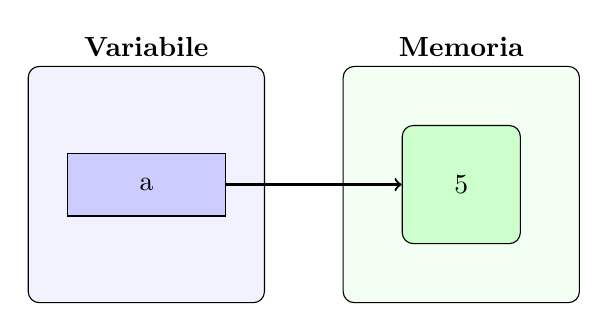
\begin{tikzpicture}
    % Riquadri con titoli
    \node[draw, rounded corners, fill=blue!5, minimum width=3cm, minimum height=3cm, label={[font=\bfseries]above:Variabile}] (var_box) at (0,0) {};
    
    \node[draw, rounded corners, fill=green!5, minimum width=3cm, minimum height=3cm, label={[font=\bfseries]above:Memoria}] (mem_box) at (4,0) {};
    
    % Variabile
    \node[draw, fill=blue!20, minimum width=2cm, minimum height=0.8cm] (var_a) at (0,0) {a};
    
    % Oggetto in memoria
    \node[draw, fill=green!20, minimum width=1.5cm, minimum height=1.5cm, rounded corners] (obj_5) at (4,0) {5};
    
    % Freccia di riferimento
    \draw[->, thick] (var_a) -- (obj_5);
\end{tikzpicture}
\end{center}

Python crea un oggetto intero con valore 5 in memoria e associa la variabile \texttt{a} a questo oggetto.\\ La variabile \texttt{a} non "contiene" 5, ma "punta a" o "fa riferimento a" l'oggetto 5 in memoria.

\subsection{Assegnazione di variabili}

Vediamo cosa succede quando creiamo una seconda variabile e le assegniamo il valore della prima:

\begin{lstlisting}
a = 5
b = a  # b ora fa riferimento allo stesso oggetto di a
\end{lstlisting}

\begin{center}
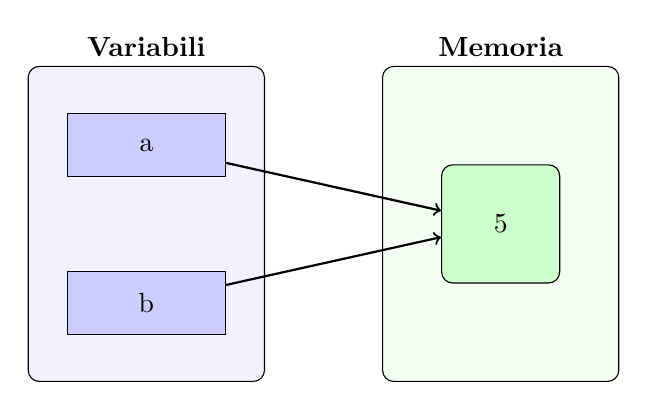
\begin{tikzpicture}
    % Riquadri di raggruppamento
    \node[draw, rounded corners, fill=blue!5, minimum width=3cm, minimum height=4cm, label={[font=\bfseries]above:Variabili}] (vars) at (0,0) {};
    \node[draw, rounded corners, fill=green!5, minimum width=3cm, minimum height=4cm, label={[font=\bfseries]above:Memoria}] (mem) at (4.5,0) {};
    
    % Variabili
    \node[draw, fill=blue!20, minimum width=2cm, minimum height=0.8cm] (var_a) at (0,1) {a};
    \node[draw, fill=blue!20, minimum width=2cm, minimum height=0.8cm] (var_b) at (0,-1) {b};
    
    % Oggetto in memoria
    \node[draw, fill=green!20, minimum width=1.5cm, minimum height=1.5cm, rounded corners] (obj_5) at (4.5,0) {5};
    
    % Frecce di riferimento
    \draw[->, thick] (var_a) -- (obj_5);
    \draw[->, thick] (var_b) -- (obj_5);
\end{tikzpicture}
\end{center}

Ora sia \texttt{a} che \texttt{b} fanno riferimento allo stesso oggetto in memoria. Non viene creata una copia del valore.

\subsection{Tipi immutabili vs mutabili}\label{mutableImmutable}
    In Python, la distinzione tra tipi di dati mutabili e immutabili rappresenta uno dei concetti fondamentali che influenzano profondamente il comportamento del codice. Questa distinzione, apparentemente semplice, ha implicazioni significative sulla manipolazione dati, sull'ottimizzazione della memoria.

    \subsubsection*{La natura dell'immutabilità e della mutabilità}
    Quando parliamo di \textbf{immutabilità}, ci riferiamo a oggetti che, una volta creati, non possono essere modificati nel loro stato interno. Qualsiasi opeazione sembra modificare un oggetto immutabile in realtà crea un nuovo oggetto con i valori aggiornati. È come se questi oggetti portassero con sé un cartello invisibile che dice: "Guardami, ma non toccarmi".
    Al contrario, gli oggetti mutabili possono essere alterati dopo la loro creazione. Il loro stato interno può cambiare mentre l'identità dell'oggetto rimane la stessa. Possiamo pensare agli oggetti mutabili come a contenitori il cui contenuto può essere modificato, rimosso o sostituito senza dover sostituire l'intero contenitore.

    \subsubsection*{La classificazione In Python}
    Python organizza i suoi tipi di dati nativi in queste due categorie:

    \begin{itemize}
        \item \textbf{Tipi Immutabili:}
        \begin{itemize}
            \item \textbf{Numeri} (\textit{int, float, complex})
            \item \textbf{Stringe} (\textit{str})
            \item \textbf{Tuple} (\textit{tuple})
            \item \textbf{Frozen sets} (\textit{frozenset})
            \item \textbf{Booleani} (\textit{bool})
            \item \textbf{None} (\textit{NoneType})
        \end{itemize}
    \end{itemize}

    \begin{itemize}
        \item \textbf{Tipi Mutabili:}
        \begin{itemize}
            \item \textbf{Liste} (\textit{list})
            \item \textbf{Dizionari} (\textit{dict})
            \item \textbf{Set} (\textit{set})
        \end{itemize}
    \end{itemize}

    \subsubsection*{Un modello concettuale}
    Per comprendere meglio questa distinzione, possiamo utilizzare un'analogia:

    Gli oggetti \textbf{immutabili} sono come documenti stampati su carta: se desideri modificare una parola, devi creare un nuovo documento. Non puoi alterare l'originale senza lasciare tracce evidenti.

    Gli oggetti \textbf{mutabili} sono invece come documenti digitali prima della stampa, alla quale puoi ancora aggiungere, eliminare o modificare i contenuti, mantenendo lo stesso file.
\vspace{0,5cm}
    

\begin{tcolorbox}[colback=blue!5!white,colframe=blue!75!black,title=Differenza tra tipi immutabili e mutabili]\label{TabellaMutabilitàImmutabilità}
In Python, la distinzione tra tipi immutabili e mutabili è fondamentale per comprendere il comportamento delle variabili:

\begin{itemize}[leftmargin=*,itemsep=0.5em]
    \item \textbf{Tipi immutabili} (non modificabili dopo la creazione):
    \begin{itemize}
        \item \texttt{int}: Numeri interi
        \item \texttt{float}: Numeri in virgola mobile
        \item \texttt{bool}: Valori booleani (True/False)
        \item \texttt{str}: Stringhe di testo
        \item \texttt{tuple}: Sequenze immutabili di elementi
        \item \texttt{frozenset}: Insiemi immutabili
    \end{itemize}
    
    \item \textbf{Tipi mutabili} (modificabili dopo la creazione):
    \begin{itemize}
        \item \texttt{list}: Liste di elementi
        \item \texttt{dict}: Dizionari (coppie chiave-valore)
        \item \texttt{set}: Insiemi di elementi unici
    \end{itemize}
\end{itemize}

Questa distinzione influenza profondamente come le variabili si comportano quando vengono assegnate, passate a funzioni o modificate.
\end{tcolorbox}

\subsubsection{Comportamento con tipi immutabili}

Quando lavoriamo con tipi immutabili, qualsiasi operazione che sembra modificare il valore in realtà crea un nuovo oggetto in memoria:

\begin{lstlisting}
a = 5
b = a
a = 10  # Questo NON modifica l'oggetto originale, ma crea un nuovo riferimento
print(b)  # Output: 5 (b continua a riferirsi all'oggetto originale)
\end{lstlisting}
\subsubsection{Comportamento con tipi mutabili}

I tipi mutabili come le liste si comportano diversamente:

\begin{lstlisting}
lista_a = [1, 2, 3]
lista_b = lista_a
lista_a.append(4)  # Questo modifica l'oggetto originale a cui puntano entrambe le variabili
\end{lstlisting}

Stato iniziale:
\begin{center}
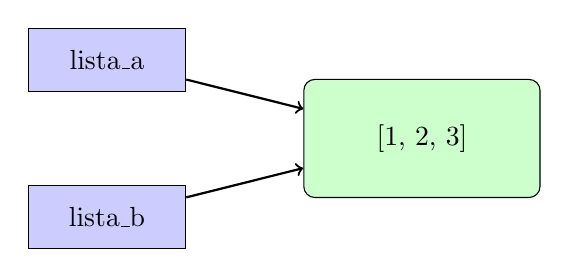
\begin{tikzpicture}
    % Variabili
    \node[draw, fill=blue!20, minimum width=2cm, minimum height=0.8cm] (var_a) at (0,1) {lista\_a};
    \node[draw, fill=blue!20, minimum width=2cm, minimum height=0.8cm] (var_b) at (0,-1) {lista\_b};
    
    % Oggetto in memoria
    \node[draw, fill=green!20, minimum width=3cm, minimum height=1.5cm, rounded corners] (obj_list) at (4,0) {[1, 2, 3]};
    
    % Frecce di riferimento
    \draw[->, thick] (var_a) -- (obj_list);
    \draw[->, thick] (var_b) -- (obj_list);
\end{tikzpicture}
\end{center}

Dopo \texttt{lista\_a.append(4)}:
\begin{center}
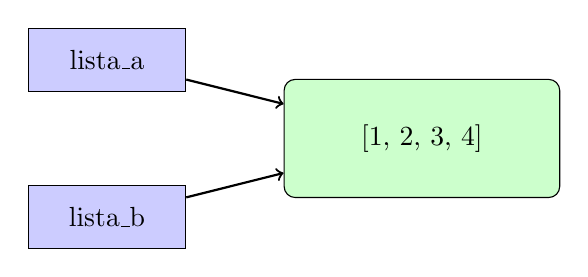
\begin{tikzpicture}
    % Variabili
    \node[draw, fill=blue!20, minimum width=2cm, minimum height=0.8cm] (var_a) at (0,1) {lista\_a};
    \node[draw, fill=blue!20, minimum width=2cm, minimum height=0.8cm] (var_b) at (0,-1) {lista\_b};
    
    % Oggetto in memoria modificato
    \node[draw, fill=green!20, minimum width=3.5cm, minimum height=1.5cm, rounded corners] (obj_list) at (4,0) {[1, 2, 3, 4]};
    
    % Frecce di riferimento
    \draw[->, thick] (var_a) -- (obj_list);
    \draw[->, thick] (var_b) -- (obj_list);
\end{tikzpicture}
\end{center}

In questo caso, \texttt{lista\_a.append(4)} modifica direttamente l'oggetto lista in memoria. Poiché sia \texttt{lista\_a} che \texttt{lista\_b} puntano allo stesso oggetto, entrambe "vedono" la modifica.

\subsection{Verifica dell'identità degli oggetti}

Python fornisce due operatori per confrontare le variabili:

\textit{consultare per ripasso la sezione degli Operatori logici: \textbf{\nameref{opLogici}}}
\begin{itemize}
    \item \texttt{==} confronta i valori (uguaglianza)
    \item \texttt{is} confronta le identità (se le variabili puntano allo stesso oggetto)
\end{itemize}

\begin{lstlisting}
a = [1, 2, 3]
b = [1, 2, 3]  # Una nuova lista con gli stessi valori
c = a          # Riferimento alla stessa lista

print(a == b)  # True (stesso valore)
print(a is b)  # False (oggetti diversi)
print(a is c)  # True (stesso oggetto)

# Possiamo verificare l'identita anche con id()
print(id(a))  # Un numero unico che identifica l'oggetto
print(id(b))  # Un numero diverso
print(id(c))  # Stesso numero di id(a)
\end{lstlisting}

\begin{center}
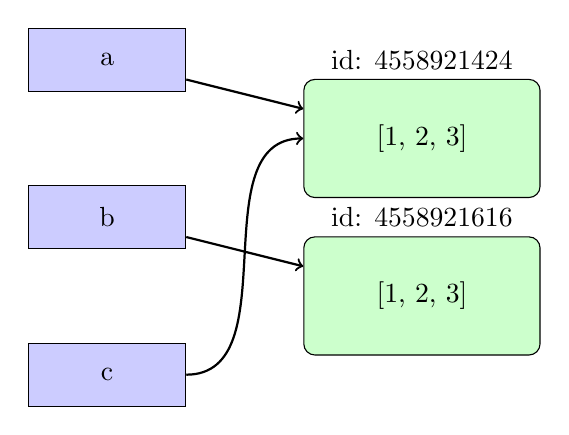
\begin{tikzpicture}
    % Variabili
    \node[draw, fill=blue!20, minimum width=2cm, minimum height=0.8cm] (var_a) at (0,2) {a};
    \node[draw, fill=blue!20, minimum width=2cm, minimum height=0.8cm] (var_b) at (0,0) {b};
    \node[draw, fill=blue!20, minimum width=2cm, minimum height=0.8cm] (var_c) at (0,-2) {c};
    
    % Oggetti in memoria
    \node[draw, fill=green!20, minimum width=3cm, minimum height=1.5cm, rounded corners] (obj_list1) at (4,1) {[1, 2, 3]};
    \node[draw, fill=green!20, minimum width=3cm, minimum height=1.5cm, rounded corners] (obj_list2) at (4,-1) {[1, 2, 3]};
    
    % Frecce di riferimento
    \draw[->, thick] (var_a) -- (obj_list1);
    \draw[->, thick] (var_b) -- (obj_list2);
    \draw[->, thick] (var_c) to [out=0,in=180] (obj_list1);
    
    % IDs
    \node[above] at (obj_list2.north) {id: 4558921616};
    \node[above] at (obj_list1.north) {id: 4558921424};
\end{tikzpicture}
\end{center}

\subsection{Esercizio pratico: tracciare le variabili}

Esaminiamo un esercizio completo che mostra come tracciare le variabili in Python. Prevedere l'output di questo programma richiede di comprendere come Python gestisce i riferimenti in memoria.

\begin{lstlisting}
# Stato iniziale
x = 10
y = x
lista = [1, 2]
dizionario = {'a': 1, 'b': 2}

# Modifichiamo le variabili
x = 20
lista.append(3)
dizionario['c'] = 3

# Verifichiamo lo stato finale
print(x)        # Output: 20
print(y)        # Output: 10
print(lista)    # Output: [1, 2, 3]
print(dizionario)  # Output: {'a': 1, 'b': 2, 'c': 3}
\end{lstlisting}

Visualizziamo lo stato della memoria in diversi momenti dell'esecuzione:

\textbf{Stato iniziale:}
\begin{center}
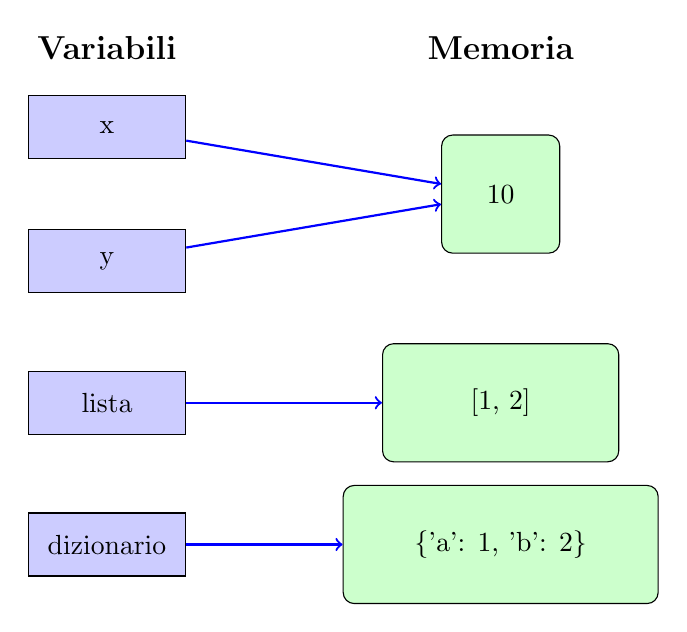
\begin{tikzpicture}
    % Etichette per le sezioni con maggiore evidenza
    \node[align=center, font=\bfseries\large] at (0,3.5) {Variabili};
    \node[align=center, font=\bfseries\large] at (5,3.5) {Memoria};
    
    % Variabili - maggiore spaziatura verticale
    \node[draw, fill=blue!20, minimum width=2cm, minimum height=0.8cm] (var_x) at (0,2.5) {x};
    \node[draw, fill=blue!20, minimum width=2cm, minimum height=0.8cm] (var_y) at (0,0.8) {y};
    \node[draw, fill=blue!20, minimum width=2cm, minimum height=0.8cm] (var_lista) at (0,-1.0) {lista};
    \node[draw, fill=blue!20, minimum width=2cm, minimum height=0.8cm] (var_dict) at (0,-2.8) {dizionario};
    
    % Oggetti in memoria - più distanziati e spostati a destra
    \node[draw, fill=green!20, minimum width=1.5cm, minimum height=1.5cm, rounded corners] (obj_10) at (5,1.65) {10};
    \node[draw, fill=green!20, minimum width=3cm, minimum height=1.5cm, rounded corners] (obj_lista) at (5,-1.0) {[1, 2]};
    \node[draw, fill=green!20, minimum width=4cm, minimum height=1.5cm, rounded corners] (obj_dict) at (5,-2.8) {\{'a': 1, 'b': 2\}};
    
    % Frecce di riferimento più eleganti
    \draw[->, thick, blue] (var_x) -- (obj_10);
    \draw[->, thick, blue] (var_y) -- (obj_10);
    \draw[->, thick, blue] (var_lista) -- (obj_lista);
    \draw[->, thick, blue] (var_dict) -- (obj_dict);
\end{tikzpicture}
\end{center}

\textbf{Dopo x = 20:}
\begin{center}
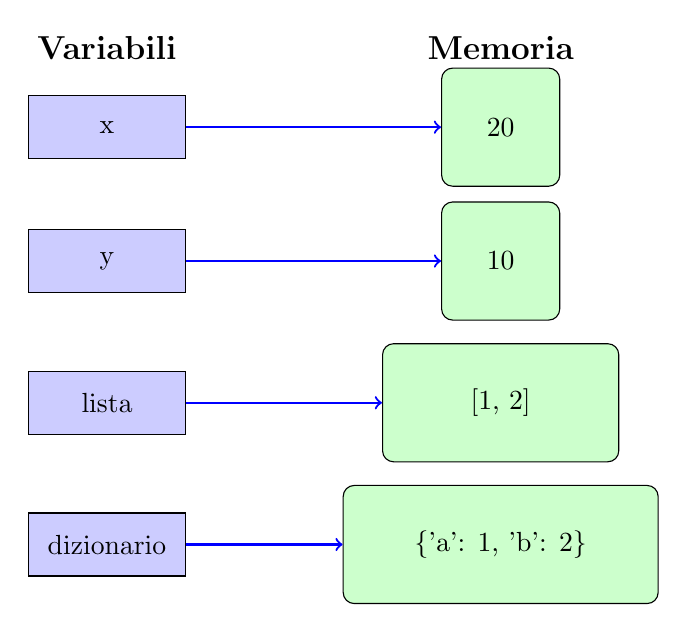
\begin{tikzpicture}
    % Etichette per le sezioni
    \node[align=center, font=\bfseries\large] at (0,3.5) {Variabili};
    \node[align=center, font=\bfseries\large] at (5,3.5) {Memoria};
    
    % Variabili - maggiore spaziatura verticale
    \node[draw, fill=blue!20, minimum width=2cm, minimum height=0.8cm] (var_x) at (0,2.5) {x};
    \node[draw, fill=blue!20, minimum width=2cm, minimum height=0.8cm] (var_y) at (0,0.8) {y};
    \node[draw, fill=blue!20, minimum width=2cm, minimum height=0.8cm] (var_lista) at (0,-1.0) {lista};
    \node[draw, fill=blue!20, minimum width=2cm, minimum height=0.8cm] (var_dict) at (0,-2.8) {dizionario};
    
    % Oggetti in memoria - più distanziati e spostati a destra
    \node[draw, fill=green!20, minimum width=1.5cm, minimum height=1.5cm, rounded corners] (obj_20) at (5,2.5) {20};
    \node[draw, fill=green!20, minimum width=1.5cm, minimum height=1.5cm, rounded corners] (obj_10) at (5,0.8) {10};
    \node[draw, fill=green!20, minimum width=3cm, minimum height=1.5cm, rounded corners] (obj_lista) at (5,-1.0) {[1, 2]};
    \node[draw, fill=green!20, minimum width=4cm, minimum height=1.5cm, rounded corners] (obj_dict) at (5,-2.8) {\{'a': 1, 'b': 2\}};
    
    % Frecce di riferimento più eleganti
    \draw[->, thick, blue] (var_x) -- (obj_20);
    \draw[->, thick, blue] (var_y) -- (obj_10);
    \draw[->, thick, blue] (var_lista) -- (obj_lista);
    \draw[->, thick, blue] (var_dict) -- (obj_dict);
\end{tikzpicture}
\end{center}

\textbf{Stato finale (dopo tutte le modifiche):}
\begin{center}
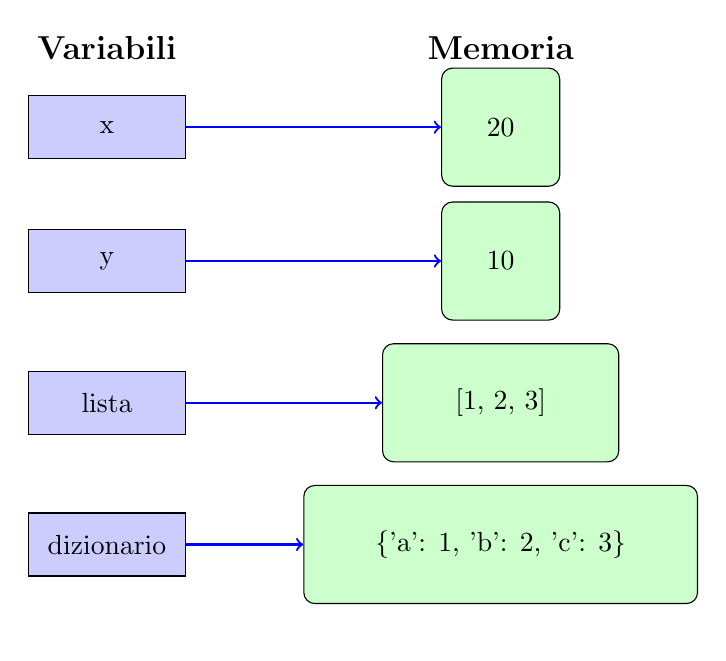
\begin{tikzpicture}
    % Etichette per le sezioni
    \node[align=center, font=\bfseries\large] at (0,3.5) {Variabili};
    \node[align=center, font=\bfseries\large] at (5,3.5) {Memoria};
    
    % Variabili - maggiore spaziatura verticale
    \node[draw, fill=blue!20, minimum width=2cm, minimum height=0.8cm] (var_x) at (0,2.5) {x};
    \node[draw, fill=blue!20, minimum width=2cm, minimum height=0.8cm] (var_y) at (0,0.8) {y};
    \node[draw, fill=blue!20, minimum width=2cm, minimum height=0.8cm] (var_lista) at (0,-1.0) {lista};
    \node[draw, fill=blue!20, minimum width=2cm, minimum height=0.8cm] (var_dict) at (0,-2.8) {dizionario};
    
    % Oggetti in memoria - più distanziati e spostati a destra
    \node[draw, fill=green!20, minimum width=1.5cm, minimum height=1.5cm, rounded corners] (obj_20) at (5,2.5) {20};
    \node[draw, fill=green!20, minimum width=1.5cm, minimum height=1.5cm, rounded corners] (obj_10) at (5,0.8) {10};
    \node[draw, fill=green!20, minimum width=3cm, minimum height=1.5cm, rounded corners] (obj_lista) at (5,-1.0) {[1, 2, 3]};
    \node[draw, fill=green!20, minimum width=5cm, minimum height=1.5cm, rounded corners] (obj_dict) at (5,-2.8) {\{'a': 1, 'b': 2, 'c': 3\}};
    
    % Frecce di riferimento più eleganti
    \draw[->, thick, blue] (var_x) -- (obj_20);
    \draw[->, thick, blue] (var_y) -- (obj_10);
    \draw[->, thick, blue] (var_lista) -- (obj_lista);
    \draw[->, thick, blue] (var_dict) -- (obj_dict);
    
    % Aggiunta: cornice attorno al nuovo elemento aggiunto per evidenziare la modifica

    \node[red, font=\small\bfseries] at (5,-2.0) {};
    

    \node[red, font=\small\bfseries] at (5,-3.8) {};
\end{tikzpicture}
\end{center}

Nota come:
\begin{itemize}
    \item \texttt{x} punta a un nuovo oggetto (20), mentre \texttt{y} continua a puntare all'oggetto originale (10)
    \item Gli oggetti mutabili (\texttt{lista} e \texttt{dizionario}) sono stati modificati in memoria, non è stato creato un nuovo oggetto
    \item Tutte le variabili che puntano a oggetti mutabili vedono le modifiche apportate
\end{itemize}

Questo esercizio illustra la differenza fondamentale tra l'assegnazione di nuovi valori (che crea nuovi riferimenti per tipi immutabili) e la modifica di oggetti mutabili (che altera gli oggetti esistenti in memoria).


